\documentclass[a4paper, 12pt]{article}
\usepackage{graphicx} % Required for inserting images
\usepackage[left=3cm, top=3cm, right=2cm, bottom=2cm]{geometry}
\usepackage{setspace}
\onehalfspacing
\usepackage{indentfirst}
\usepackage{float}
\usepackage[hidelinks]{hyperref}
\graphicspath{ {./images/} }
\usepackage{minted}
\usepackage{caption}
\usepackage{titlesec}
\usepackage{makecell}
\usepackage{booktabs}
\usepackage{array}
\usepackage{longtable}
\usepackage{enumitem}
\usepackage{listings}
\usepackage{xcolor}
\usepackage[style=abnt, backend=biber]{biblatex}
\addbibresource{referencias.bib}

\lstset{
  basicstyle=\ttfamily\tiny,
  keywordstyle=\color{blue},
  commentstyle=\color{green!50!black},
  stringstyle=\color{red},
  numbers=left,
  numberstyle=\tiny,
  stepnumber=1,
  numbersep=8pt,
  showstringspaces=false,
  breaklines=true,
  frame=single,
  tabsize=4
}
% Define o tamanho da section para \small (pequeno) e negrito (\bfseries)




% formatação da numeração de páginas
\usepackage{fancyhdr}
\pagestyle{fancy}
\fancyhf{}
\fancyhead[R]{\thepage}
\renewcommand{\headrulewidth}{0pt}


\begin{document}

% CAPA ========================================
\begin{center}

    \thispagestyle{empty}
    
    \textbf{UNIVERSIDADE FEDERAL DO RIO GRANDE DO SUL}\\
    \textbf{INSTITUTO DE INFORMATICA}\\
    \vspace{3cm}

    \textbf{GABRIEL ALEXANDRE RICHTER}\\
    \textbf{GUSTAVO MACHADO SILVA}\\
    \textbf{LUCAS GOMES DE SOUZA}\\
    \textbf{MAURI DELGADO HERNANDEZ}\\
    \textbf{YASMIN AGNES SIMÃO}\\
    \vspace{4cm}
    
    \textbf{TRABALHO PRÁTICO}\\
    \textbf{Sprint 02 - Modelagem e Arquitetura}\\
    \vspace{5cm}

    \textbf{Disciplina: Engenharia de Software N (INF01127)}\\
    \textbf{Professora: Leticia dos Santos Machado}\\
    \vspace{5cm}

    \textbf{Porto Alegre, abril de 2026.}\\
    
\end{center}

% contents
\newpage
\thispagestyle{empty}
\tableofcontents


% SECTIONS ==================================
\newpage
\section{INTRODUÇÃO}
O envelhecimento da população tem ampliado a necessidade de soluções que apoiem a manutenção da autonomia, do bem-estar e da integração social das pessoas idosas. 
Muitas organizações comunitárias e ONGs promovem atividades físicas, cognitivas e sociais voltadas a esse público, porém enfrentam desafios para manter a participação contínua dos membros, especialmente quando as interações dependem de encontros presenciais. Nesse contexto, surge a oportunidade de desenvolver uma plataforma digital que permita que pessoas idosas participem de atividades online e interajam com outros membros da comunidade.
A solução deve considerar características importantes desse público, como facilidade de uso, clareza visual, entre outras, promovendo experiências positivas de interação, reduzindo barreiras tecnológicas e fortalecendo o senso de pertencimento à comunidade. 
Além dos participantes idosos, há também o papel de mediadores comunitários (tutores), responsáveis por organizar atividades, compartilhar conteúdos e estimular a participação dos membros. A tecnologia deve apoiar esses mediadores na gestão das atividades e na comunicação com o grupo, garantindo que as interações ocorram de forma organizada e
segura.
A partir dessa narrativa inicial, o seguinte trabalho explora possíveis funcionalidades, as necessidades dos usuários e os requisitos do sistema, considerando aspectos de usabilidade, acessibilidade, interação social, suporte tecnológico e gestão das atividades.
\newpage
\section{DESK RESEARCH}
Segundo IBGE (2022), o número de adultos com 65 anos ou mais chegou perto de 22,2 milhões, o que representa cerca de 10,9\% da população e um crescimento de 57,4\% em relação a 2010. Também de acordo com o IBGE, a porcentagem de pessoas 60+ que utilizam a internet em seu dia a dia foi de 66\% em 2023.
O observatório Febraban de 2022 realizou uma pesquisa sobre inclusão digital de idosos no país, os resultados apontam um crescimento desta inclusão, 64\% dos cerca de 450 idosos respondentes dizem que fazem uso regular de internet. O celular foi eleito como dispositivo mais utilizado (90\%), e os principais usos são para comunicação (redes sociais e videochamadas), entretenimento (redes digitais e plataformas de streaming), pesquisa de produtos e preços e uso de serviços bancários, principalmente o PIX. As principais dificuldades relatadas é a falta de familiaridade, também relacionada com interfaces complexas e/ou pouco amigáveis, medo de cometer erros durante o uso e insegurança com fraudes e golpes, 70\% responderam que não se sentem seguros online (FEBRABAN, 2022).


No Brasil existem várias iniciativas que promovem a interação social para idosos, com o objetivo de melhorar a qualidade de vida. A principal delas é o SESC, que é referência nacional e está presente em todos os estados. Vale também mencionar outras organizações, como o Instituto Velho Amigo em São Paulo, como foco em idosos em situação de vulnerabilidade social, a Associação dos Amigos dos Idosos do Brasil em Aracaju e o Núcleo de Convivência de Idoso, também em São Paulo


 No Brasil existe um movimento de preocupação com o bem estar das pessoas com mais de 65 anos, podemos ver a partir da quantidade de iniciativas nesse sentido, entretanto a grande maioria destes  projetos são realizados de forma presencial e possuem alcance e capacidade limitados. Agora pensando no que foi dito sobre inclusão digital, idosos cada vez mais acessando e utilizando recursos de internet, existe um potencial de juntar estas soluções. Realizar iniciativas de interação social em ambientes digitais vai aumentar seu alcance e capacidade de atendimento, impactando positivamente muitas mais vidas.

\newpage
\section{BENCHMARK}
Através da pesquisa de soluções já existentes no mercado, descobrimos que as soluções atuais focam em acessibilidade visual (botões grandes, interfaces limpas) e em conectar a pessoa idosa à sua família ou a cuidadores de forma individualizada. A maioria das plataformas analisadas falha no aspecto comunitário e de gestão logística. O nosso cenário descreve um sistema que empodera mediadores/tutores comunitários a gerenciarem grupos, criarem atividades sociais e acompanhar relatórios de parcipação. Nenhuma das plataformas pesquisadas possui a combinação de:

\begin{enumerate}
    \item Painel administrativo para criação e gestão de inscrições em atividades.
    \item Ambiente de grupo seguro e mediado.
    \item Videochamadas nativas integradas à agenda da comunidade.
\end{enumerate}

Apresentamos um resumo das plataformas pesquisadas nos próximos tópicos.

\subsection{Projeto Rede Bem Estar (App Madu - Instituto Tellus)}
Esta é uma plataforma digital (site e aplicativo) focada em entregar conteúdos relevantes sobre o envelhecimento para idosos, familiares e cuidadores, com o objetivo de fortalecer vínculos e quebrar estereótipos.

\begin{itemize}
    \item \textbf{Requisitos Funcionais Contemplados}
        \begin{itemize}
            \item Acesso a conteúdos compartilhados: O app possui categorias de notícias, dicas de saúde, finanças e vídeos.
            \item Lembretes automáticos: Possui um sistema de notificações a cada três dias baseado nos interesses do usuário.
            \item Cadastro de usuários: Permite criação de perfil para personalização de conteúdo.
        \end{itemize}
    \item \textbf{Requisitos Funcionais NÃO Contemplados}
        \begin{itemize}
            \item Não possui visualização ou inscrição em atividades ao vivo.
            \item Não possui ferramenta nativa para videochamadas.
            \item Não permite troca de mensagens em grupo dentro do app (no projeto piloto, utilizaram o WhatsApp à parte).
            \item Não possui painel de gestão para mediadores criarem/editarem atividades ou gerenciarem listas de participantes.
        \end{itemize}
    \item \textbf{Requisitos Não-Funcionais Contemplados}
        \begin{itemize}
            \item Interface simples e intuitiva: Foco em baixa complexidade e facilidade de leitura.
            \item Funciona em celulares, tablets e computadores: Possui versão web, iOS e Android.
            \item Compatibilidade de acessibilidade: O site conta com o widget VLibras.
        \end{itemize}
    \item \textbf{Diferenciais / Funcionalidades Extras}
        \begin{itemize}
            \item \textbf{Identidade visual humanizada:} Uso da persona "Madu" para gerar conexão com o usuário.
            \item \textbf{Kit do Gestor:} Um programa educativo e materiais de formação (online e impresso) voltado para capacitar facilitadores e gestores de grupos de idosos, o que dialoga muito com a sua ideia de "mediadores comunitários".
        \end{itemize}
\end{itemize}

\subsection{Memoryboard}
Trata-se de um quadro de mensagens digital em formato de hardware (um display de 10 ou 15 polegadas) que fica na casa do idoso. A família gerencia o que aparece na tela por meio de um aplicativo remoto.

\begin{itemize}
    \item \textbf{Requisitos Funcionais Contemplados}
        \begin{itemize}
            \item Acesso a conteúdos compartilhados: Recebe fotos e mensagens.
            \item Lembretes automáticos: A família pode programar lembretes (ex: "hora do remédio").
            \item Troca de mensagens: Recebe mensagens de familiares.
        \end{itemize}
    \item \textbf{Requisitos Funcionais NÃO Contemplados}
        \begin{itemize}
            \item A comunicação é praticamente unilateral (da família para o idoso). Não há inscrição em atividades comunitárias, chat entre vários idosos, videochamadas integradas ou gestão de grupos.
        \end{itemize}
    \item \textbf{Requisitos Não-Funcionais Contemplados}
        \begin{itemize}
            \item Interface simples e intuitiva: Extrema facilidade de uso, pois o idoso não precisa interagir tecnicamente com o aparelho.
            \item Textos legíveis: Design focado em exibição clara e direta.
        \end{itemize}
    \item \textbf{Diferenciais / Funcionalidades Extras}
        \begin{itemize}
            \item \textbf{Remoção total da barreira tecnológica:} Como é um hardware dedicado de exibição passiva, resolve o problema de idosos com severa dificuldade motora ou cognitiva que não conseguem operar um smartphone comum.
        \end{itemize}
\end{itemize}

\subsection{Oscar Senior}
Um aplicativo de comunicação projetado especificamente para adultos mais velhos, focado em segurança e chamadas simplificadas.

\begin{itemize}
    \item \textbf{Requisitos Funcionais Contemplados}
        \begin{itemize}
            \item Acesso a atividades online: Possui videochamadas nativas e intuitivas.
            \item Troca de mensagens: Permite mensagens instantâneas.
            \item Lembretes automáticos: Focado em lembretes de medicação e rotina.
        \end{itemize}
    \item \textbf{Requisitos Funcionais NÃO Contemplados}
        \begin{itemize}
            \item Não é uma plataforma de "comunidade". Faltam recursos para mediadores criarem eventos, gerenciarem inscrições e compartilharem links de atividades em grupo.
        \end{itemize}
    \item \textbf{Requisitos Não-Funcionais Contemplados}
        \begin{itemize}
            \item Interface simples e intuitiva: Botões grandes e navegação facilitada.
            \item Autenticação segura: Cria um ambiente seguro e fechado para a família.
        \end{itemize}
    \item \textbf{Diferenciais / Funcionalidades Extras}
        \begin{itemize}
            \item \textbf{Alertas de emergência (SOS):} Um botão de pânico integrado, caso o idoso precise de ajuda imediata.
        \end{itemize}
\end{itemize}

\subsection{Connect Care App}
Aplicativo focado na conexão entre o idoso, seus familiares e profissionais de saúde/cuidadores.

\begin{itemize}
    \item \textbf{Requisitos Funcionais Contemplados}
        \begin{itemize}
            \item Videochamadas e Troca de mensagens seguras.
            \item Lembretes automáticos: Notificações de saúde.
        \end{itemize}
    \item \textbf{Requisitos Funcionais NÃO Contemplados}
        \begin{itemize}
            \item Assim como o Oscar Senior, falta o módulo de "Gestão de Atividades" (criação de turmas, relatórios de participação, inscrição em eventos comunitários).
        \end{itemize}
    \item \textbf{Diferenciais / Funcionalidades Extras}
        \begin{itemize}
            \item \textbf{Agendamento de compromissos e Check-ins de bem-estar:} Funcionalidades excelentes para tutores monitorarem a saúde e o humor diário dos idosos participantes.
        \end{itemize}
\end{itemize}

\subsection{Silver Surf Web Browser}
Não é uma plataforma social, mas sim um navegador de internet adaptado para a terceira idade.

\begin{itemize}
    \item \textbf{Como atende aos requisitos:} Ele brilha nos \textbf{Requisitos Não Funcionais.} O Silver Surf atende aos requisitos de Botões grandes, textos legíveis, possibilidade de aumentar a fonte, suporte a alto contraste e navegação minimizada.
    \item \textbf{Diferenciais / Funcionalidades Extras}
        \begin{itemize}
            \item Permite que o idoso acesse outras redes sociais (como Facebook ou portais de notícias) com uma interface sobreposta que melhora a acessibilidade geral da internet. É uma excelente inspiração de UI/UX (Design de Interface) para o seu projeto.
        \end{itemize}
\end{itemize}
\newpage
\section{REQUISITOS}
\label{sec:requisitos}
Os requisitos apresentados buscam apresentar as necessidades exergadas pelo grupo em relação ao uso da plataforma por pessoas idosas e outros agentes relacionados. Os requisitos foram dividos em requisitos funcionais e não funcionais.

\subsection{Requisitos Funcionais}
Os requisitos funcionais definem os recuros que o sistema deve fornecer. Sendo eles:

\begin{itemize}
    \item \textbf{Acesso e Autenticação}
        \begin{enumerate}
            \item [US1] Como pessoa idosa com pouca experiência digital, quero acessar a plataforma em até 2 passos após abrir o aplicativo, para não me sentir confuso ou desistir do uso.
            \item [US2] Como usuário, quero recuperar minha senha de forma simples, para não ficar bloqueado fora da plataforma.
            \item [US3] Como idoso, quero acessar a plataforma com login simples (ex: botão único ou biometria), para evitar dificuldades com senhas complexas.
        \end{enumerate}
 
    \item \textbf{Visualização e Inscrição em Atividades}
        \begin{enumerate}
            \item [RF1] O sistema deve permitir que o participante visualize atividades disponíveis.
            \item [RF2] O sistema deve permitir inscrição em atividades.
        \end{enumerate}
 
    \item \textbf{Participação em Atividades}
        \begin{enumerate}
            \item [US4] Como pessoa idosa, quero participar de atividades online com apenas um clique a partir da tela inicial, para facilitar meu engajamento e evitar dificuldades técnicas.
            \item [US5] Como pessoa idosa, quero participar de atividades online (exercícios, jogos, encontros), para manter minha saúde e interação social.
            \item [RF3] O sistema deve permitir acesso a atividades online (ex: videochamada).
        \end{enumerate}
 
    \item \textbf{Videochamadas e Comunicação}
        \begin{enumerate}
            \item [US6] Como pessoa idosa, quero entrar em chamadas de vídeo automaticamente ao clicar em um botão, sem necessidade de configurações adicionais, para interagir com outras pessoas sem dificuldades técnicas.
            \item [US7] Como pessoa idosa, quero enviar mensagens de voz ou texto para outros participantes, para me comunicar de forma simples e manter vínculos sociais.
            \item [RF4] O sistema deve permitir troca de mensagens entre participantes.
            \item [RF5] O sistema deve permitir envio de mensagens em grupo.
        \end{enumerate}
 
    \item \textbf{Lembretes e Notificações}
        \begin{enumerate}
            \item [RF6] O sistema deve enviar lembretes automáticos de atividades (notificações ou áudio), para que os usuários não esqueçam dos eventos programados.
        \end{enumerate}
 
    \item \textbf{Conteúdos e Materiais}
        \begin{enumerate}
            \item [US8] Como idoso, quero acessar gravações das atividades passadas, para participar mesmo quando não puder estar presente ao vivo.
            \item [RF7] O sistema deve permitir acesso a conteúdos compartilhados.
            \item [RF8] O sistema deve permitir upload de conteúdos.
            \item [US9] Como pessoa idosa, quero acessar tutoriais simples e guiados, para aprender a usar a plataforma sem dificuldades.
        \end{enumerate}
 
    \item \textbf{Criação e Gestão de Atividades (Mediador/Tutor)}
        \begin{enumerate}
            \item [US10] Como mediador, quero criar e agendar atividades com data, horário e descrição, para organizar a participação dos membros de forma clara.
            \item [RF9] O sistema deve permitir criação e edição de atividades.
            \item [US11] Como tutor, quero poder marcar em calendário eventos comunitários com avisos, para que os membros estejam cientes do que ocorrerá.
        \end{enumerate}
 
    \item \textbf{Monitoramento e Engajamento (Mediador/Tutor)}
        \begin{enumerate}
            \item [US12] Como mediador, quero visualizar quem participou das atividades, para acompanhar o engajamento dos membros.
            \item [RF10] O sistema deve fornecer relatórios de participação.
            \item [US13] Como mediador, quero enviar mensagens motivacionais e avisos para o grupo, para estimular a participação contínua.
            \item [RF11] O sistema deve permitir gerenciar lista de participantes.
        \end{enumerate}
 
    \item \textbf{Moderação}
        \begin{enumerate}
            \item [US14] Como mediador, quero moderar interações no chat ou nas atividades, para garantir um ambiente seguro e respeitoso.
        \end{enumerate}
 
    \item \textbf{Social e Comunidade}
        \begin{enumerate}
            \item [US15] Como sênior, quero conhecer membros com gostos parecidos, para criar novas amizades.
            \item [US16] Como sênior, quero compartilhar acontecimentos do meu dia para outros membros, para que outros vejam o que estou fazendo.
            \item [US17] Como sênior, quero poder organizar eventos presenciais pela plataforma, para poder reunir membros da comunidade.
            \item [US18] Como sênior, quero poder conhecer membros que estejam localmente próximos de mim, para poder facilitar a criação de laços comunitários.
            \item [US19] Como tutor, quero poder selecionar para que membros minhas atividades são compartilhadas, para poder reunir membros com gostos semelhantes.
        \end{enumerate}
 
    \item \textbf{Gestão de Usuários (Administração)}
        \begin{enumerate}
            \item [US20] Como tutor, quero poder alterar os dados dos membros para atualizar informações dos usuários.
            \item [RF12] O sistema deve permitir cadastro e remoção de usuários.
            \item [RF13] O sistema deve controlar permissões de acesso.
            \item [RF14] O sistema deve registrar logs de atividades.
        \end{enumerate}
 
    \item \textbf{Suporte ao Usuário}
        \begin{enumerate}
            \item [US21] Como idoso, quero ter acesso a um botão de ajuda ou suporte imediato, para resolver dúvidas ou dificuldades rapidamente.
        \end{enumerate}
 
    \item \textbf{Preferências e Personalização}
        \begin{enumerate}
            \item [US22] Como idoso, quero configurar preferências (volume, tamanho da fonte, notificações), para adaptar a plataforma às minhas necessidades.
        \end{enumerate}
\end{itemize}

\subsection{Requisitos Não Funcionais}
Os requisitos não funcionais focam em atributos que o sistema deve aparesentar. Sendo eles:

\begin{itemize}
    \item \textbf{Usabilidade}
        \begin{enumerate}
            \item [RNF1] A interface deve ser simples e intuitiva, com navegação clara e direta.
            \item [RNF2] Deve-se minimizar o número de passos para ações principais.
        \end{enumerate}
 
    \item \textbf{Acessibilidade}
        \begin{enumerate}
            \item [RNF3] Deve usar botões grandes e textos legíveis (mínimo de 16px).
            \item [RNF4] Suporte a alto contraste.
            \item [RNF5] Possibilidade de aumentar fonte.
            \item [RNF6] Compatível com leitores de tela.
        \end{enumerate}
 
    \item \textbf{Desempenho}
        \begin{enumerate}
            \item [RNF7] O sistema deve carregar rapidamente mesmo em conexões lentas.
        \end{enumerate}
 
    \item \textbf{Segurança e Privacidade}
        \begin{enumerate}
            \item [RNF8] Dados dos usuários devem ser protegidos e sua privacidade garantida.
            \item [RNF9] Autenticação segura.
            \item [US23] Como idoso, quero interagir em um ambiente moderado e seguro, para evitar golpes, spam ou conteúdos inadequados.
        \end{enumerate}
 
    \item \textbf{Compatibilidade}
        \begin{enumerate}
            \item [RNF10] Deve funcionar em celulares, tablets e computadores.
        \end{enumerate}
\end{itemize}
\newpage
\section{CASOS DE USO E DIAGRAMAS}
A criação dos diagramas junto com os casos de uso foram baseados nos arquivos artefatos disponibilizados para pesquisa no trabalho. Utilizamos nossos requisitos para aperfeiçoar os diagramas disponíveis de acordo com as necessidades que estipulamos. Os três casos de uso e seus diagramas estão disponíveis a seguir.

% ----------------------------------------------------------------------------------------------------------

\subsection{Diagrama geral de casos de uso}

Na figura \ref{fig:diagramaGeral} está o diagrama que aborda os casos de uso da plataforma a ser desenvolvida. É a partir dele que serão apresentados diagramas de casos de uso mais específicos abaixo.

\begin{figure}[h]
    \centering
    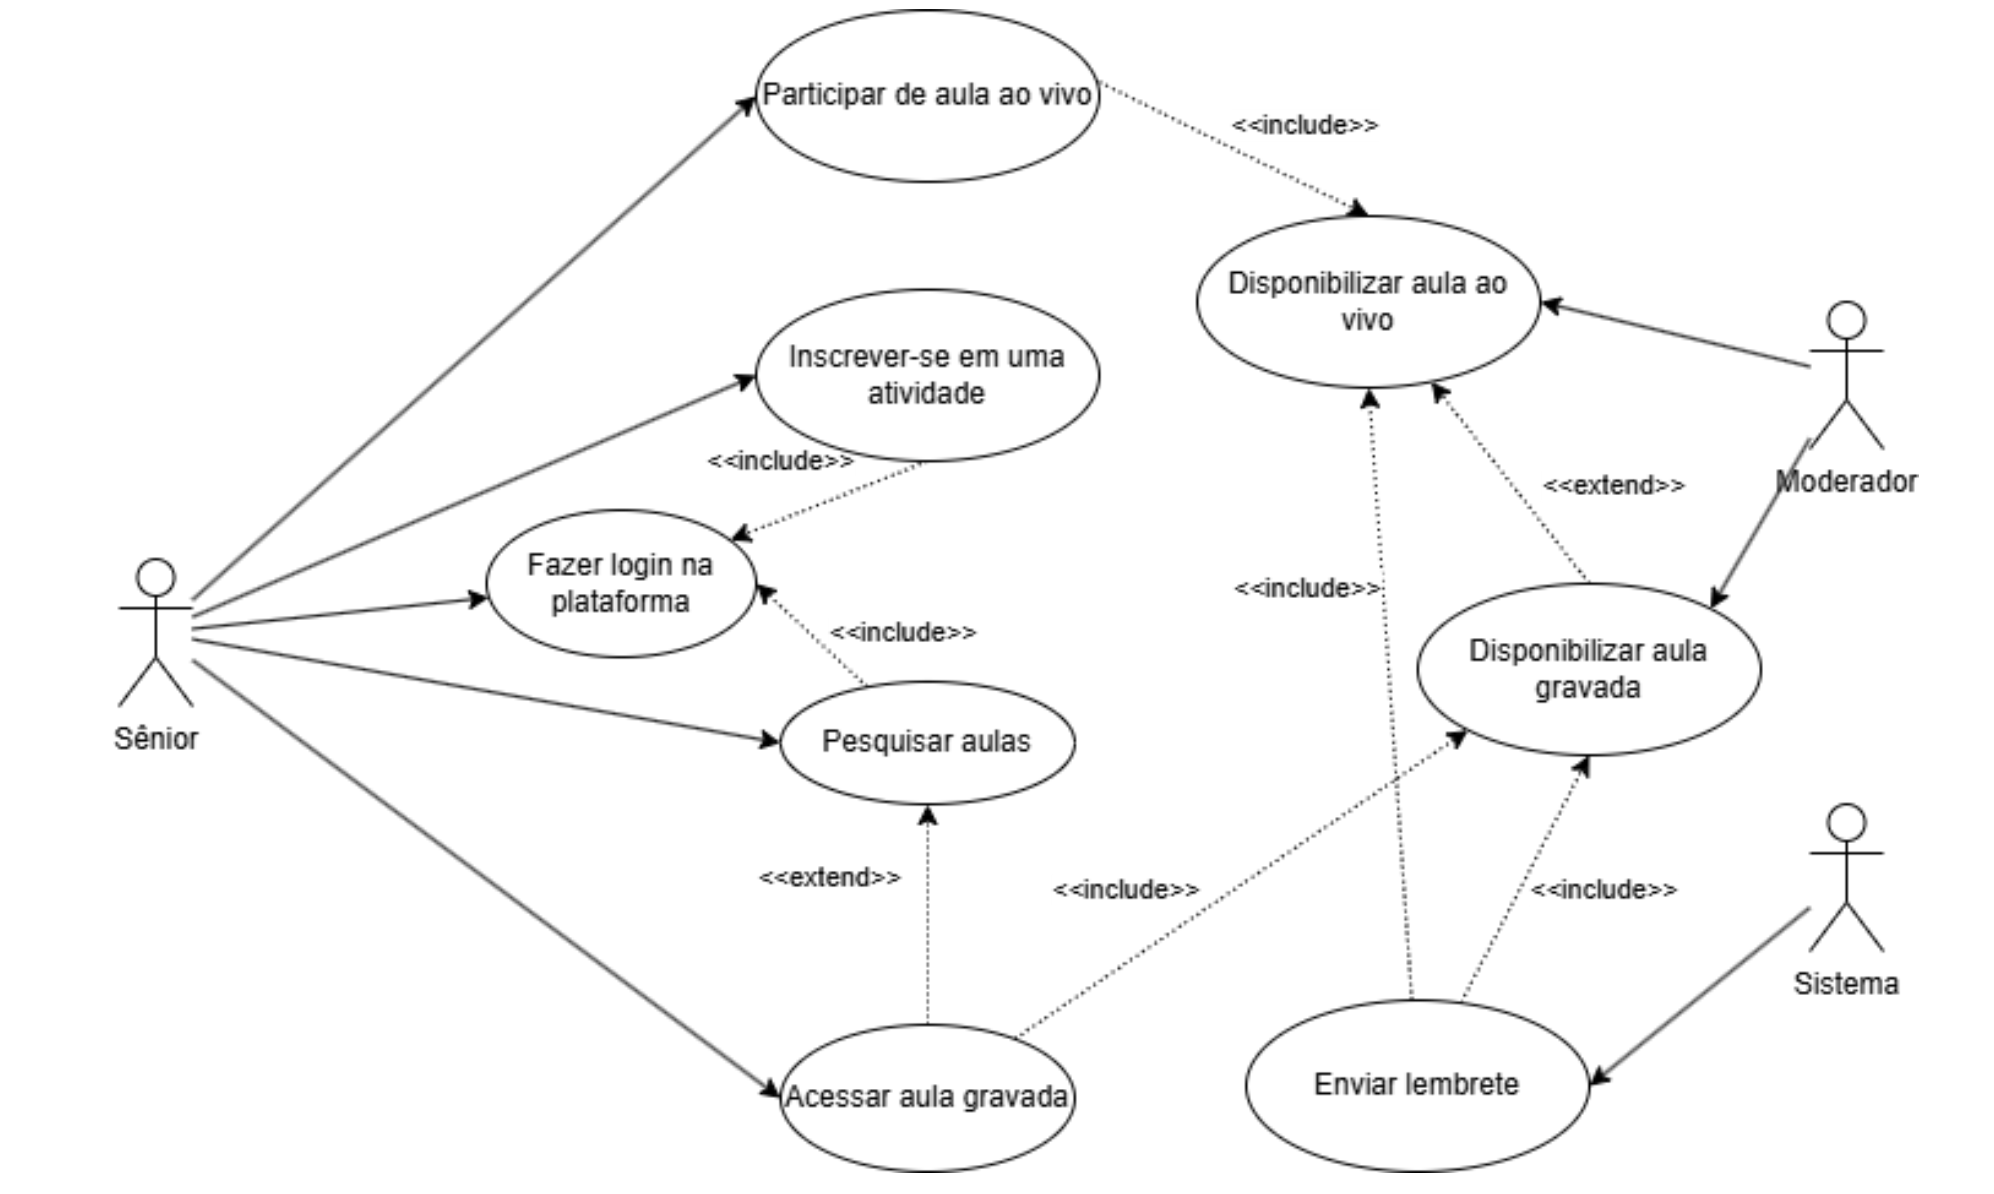
\includegraphics[width=0.8\linewidth]{images/diagramaGeral.png}
    \caption{Diagrama 1}
    \label{fig:diagramaGeral}
\end{figure}

\subsection{Assistir à aula gravada}

\begin{figure}[h]
    \centering
    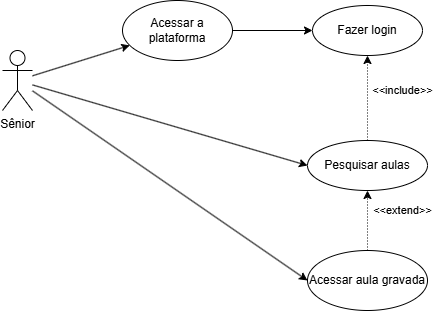
\includegraphics[width=0.8\linewidth]{images/diagrama1.png}
    \caption{Diagrama 1}
    \label{fig:diagrama1}
\end{figure}

\textbf{Atores:} Sênior

\vspace{\baselineskip}
\textbf{Descrição: } Permite ao sênior acessar a aula gravada em caso de ausência na aula síncrona.

\vspace{\baselineskip}
\textbf{Pré-condições: }
\begin{itemize}
    \item A aula gravada deve existir na plataforma.
    \item O sênior precisa estar cadastrado no sistema.
    \item O sistema que disponibiliza o vídeo deve estar funcionando.
\end{itemize}

\vspace{\baselineskip}
\textbf{Fluxo Principal: }
\begin{enumerate}
    \item O sênior acessa a plataforma;
    \item O sênior realiza o login;
    \item O sênior pesquisa as aulas disponíveis;
    \item O sênior seleciona e acessa a aula gravada desejada;
    \item O sistema carrega o vídeo e o reproduz;
\end{enumerate}

\vspace{\baselineskip}
\textbf{Fluxos Alternativos: }
\begin{itemize}
    \item 2.a - O sênior não possui cadastro na plataforma → O sistema redireciona para o cadastro.
\end{itemize}

\vspace{\baselineskip}
\textbf{Pós-condições: }
\begin{itemize}
    \item O sênior assiste à aula gravada;
    \item O vídeo fica sinalizado como assistido na plataforma;
\end{itemize}

% ----------------------------------------------------------------------------------------------------------

\subsection{Disponibilizar uma aula gravada}
\begin{figure}[H]
    \centering
    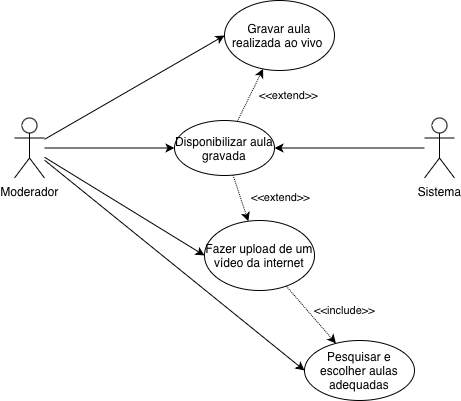
\includegraphics[width=0.8\linewidth]{images/diagrama2.png}
    \caption{Diagrama 2}
    \label{fig:diagrama2}
\end{figure}

\textbf{Atores:} Moderador, Sistema.

\vspace{\baselineskip}
\textbf{Descrição: } Permite ao moderador disponibilizar uma aula gravada para ser assistida por seniors na plataforma. Ele pode fazer isso gravando uma aula ao vivo ou pegando um vídeo da internet.

\vspace{\baselineskip}
\textbf{Pré-condições: }
\begin{itemize}
    \item Pode ou não ter acontecido uma aula ao vivo.
    \item O vídeo precisa ou não estar disponível na internet.
    \item O sistema deve estar funcionando.
\end{itemize}

\vspace{\baselineskip}
\textbf{Fluxo Principal: }
\begin{enumerate}
    \item O moderador grava a aula ao vivo que está realizando;
    \item O moderador faz upload do vídeo gravado na plataforma;
    \item O moderador disponibiliza esse vídeo para acesso dos seniors;
    \item O sistema deixa o vídeo exposto e disponível para os seniors.
\end{enumerate}

\vspace{\baselineskip}
\textbf{Fluxos Alternativos: }
\begin{itemize}
    \item 1.a - O moderador não realizou aula ao vivo - ele pode encontrar uma adequada na internet.
\end{itemize}

\vspace{\baselineskip}
\textbf{Pós-condições: }
\begin{itemize}
    \item Um novo vídeo é adicionado à plataforma.
    \item Os seniors são notificados da atualização.
\end{itemize}

% ----------------------------------------------------------------------------------------------------------

\subsection{Participar de encontro ao vivo}
\begin{figure}[H]
    \centering
    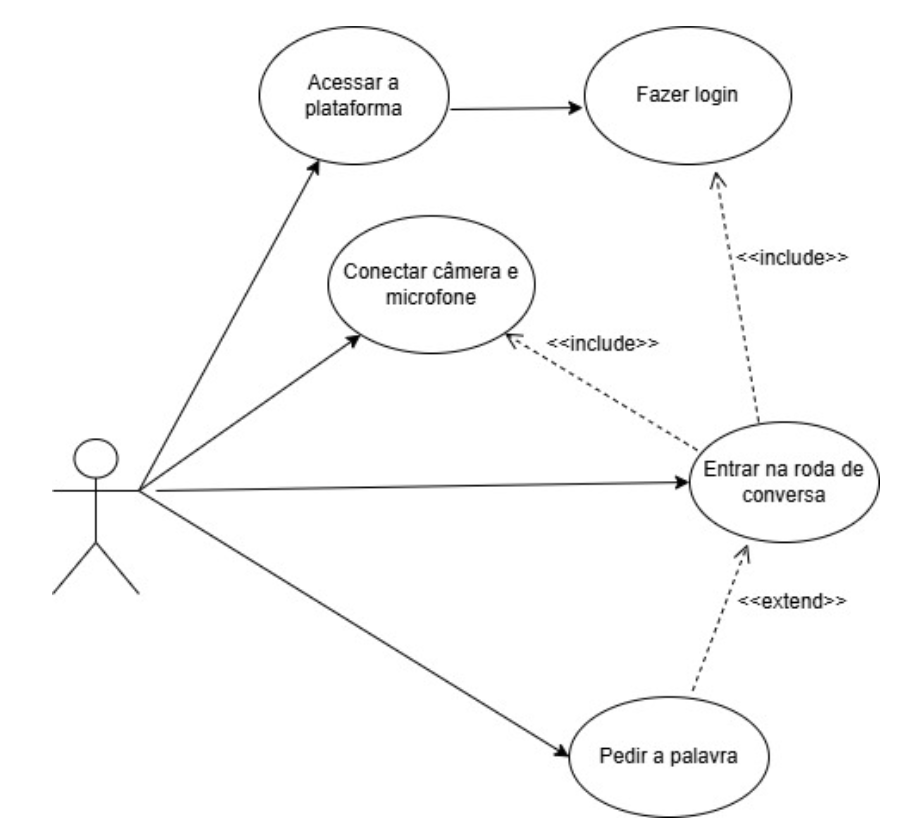
\includegraphics[width=0.8\linewidth]{images/diagrama3.png}
    \caption{Diagrama 3}
    \label{fig:diagrama3}
\end{figure}

\textbf{Atores:} Sênior

\vspace{\baselineskip}
\textbf{Descrição: } Permite ao sênior acessar e assistir a um encontro que está sendo transmitido em tempo real na plataforma. Ele pode ingressar na sala virtual, acompanhar o conteúdo e interagir durante a transmissão. 

\vspace{\baselineskip}
\textbf{Pré-condições: }
\begin{itemize}
    \item O sênior deve estar logado na plataforma.
    \item O sistema deve estar funcionando com a infraestrutura de transmissão de vídeo ativa. 
\end{itemize}

\vspace{\baselineskip}
\textbf{Fluxo Principal: }
\begin{enumerate}
    \item O sênior acessa a plataforma;
    \item O sênior realiza o login;
    \item O sênior entra no encontro ao vivo;
    \item O sistema conecta o dispositivo do sênior (áudio e vídeo) à sala de transmissão;
    \item O sistema exibe o vídeo e o áudio do encontro na tela do sênior;
    \item O sênior participa do encontro ao vivo.
\end{enumerate}

\vspace{\baselineskip}
\textbf{Fluxos Alternativos: }
\begin{itemize}
    \item 6.a - O sênior deseja interagir no encontro, pedindo a palavra,  e o sistema repassa a interação.
\end{itemize}

\vspace{\baselineskip}
\textbf{Pós-condições: }
\begin{itemize}
    \item O sênior participou e visualizou o conteúdo do encontro ao vivo. 
    \item O sistema registra a presença e o histórico de participação do sênior na plataforma.
\end{itemize}
\newpage
\section{Diagrama de Classes}
O diagrama de classes foi construído com base nos requisitos funcionais e não funcionais estipulados.
O diagrama pode ser visualizado na Figura \ref{fig:diagramaClasses}.

\begin{figure}[h]
    \centering
    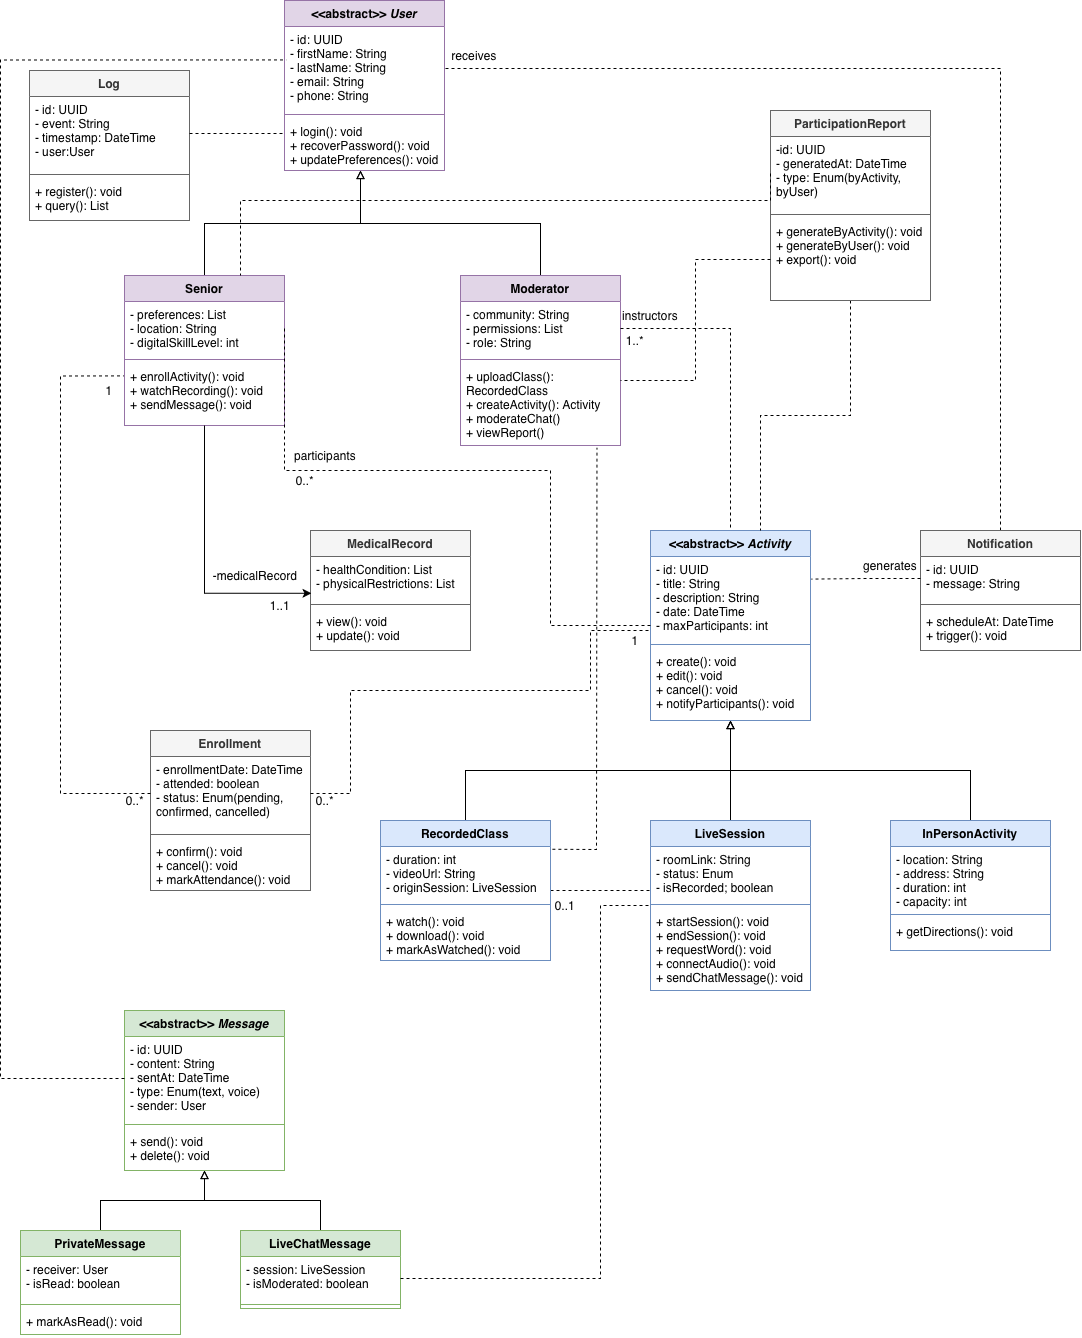
\includegraphics[width=0.8\linewidth]{images/classes_senior.png}
    \caption{Diagrama de Classes}
    \label{fig:diagramaClasses}
\end{figure}
\newpage
\section{Arquitetura}
Para esse projeto, decidimos seguir com uma arquitetura de camadas. O motivo da escolha foi devido a clareza estrutural que essa arquitetura apresenta, possibilitando uma facilidade na manutenção e adequação ao escopo do projeto.
O projeto possui responsabilidades bem distintas e a separação em camadas com cada uma tendo um escopo bem definido, ajuda a diminuir o acoplamento entre módulos e a evolução independente de cada parte do sistema.

\begin{itemize}
    \item \textbf{Camada de Apresentação (Frontend)}: Para a camada de apresentação as tecnologias escolhidas foram o framework React para desenvolvimento web e o framework React Native para desenvolvimento mobile (multiplataforma). Ambos os frameworks podem ser utilizados com a linguagem JavaScript, o que facilita na hora de compartilhar lógicas e funções.
    \item \textbf{Camada de Aplicação (Backend/API)}: Para a camada de aplicação, optamos pela utilização do Python devido ao time ter mais afinidade com a linguagem. O framework escolhido foi o Django pois funciona bem para a criação de API REST e já possui suporte para WebSocket para o chat ao vivo vida Django Channels.
    \item \textbf{Camada de Negócio (Business Logic)}: Essa camada tem como função isolar as regras de negócio da aplicação.
    \item \textbf{Camada de Dados}: Optamos por utilizar um banco de dados relacional pois acreditamos que se adequa melhor ao sistema que estamos propondo. Utilizaremos o PostgreSQL como banco de dados.
    \item \textbf{Integrações Externas}: Algumas ferramentas são essenciais para facilitar a implementação e isolar comportamentos.
        \begin{itemize}
            \item \textbf{Jitsi Meet}: Plataforma de videoconferência open source que pode ser integrada facilmente via SDK. Permite a personalização da interface, o que é interessante para a adaptação ao público alvo.
            \item \textbf{Firebase Cloud Messaging (FCM)}: Serviço de notificação em dispositivos móveis. O backend envia o comando para o FCM que realiza o disparo da notificação mesmo com o aplicativo fechado. Possui SDK para React Native.
            \item \textbf{AWS S3}: Serviço para armazenar arquivos em nuvem. Ideal para manter os vídeos e outros arquivos que serão disponibilizados no sistema.
        \end{itemize}
\end{itemize}

\nocite{*}
\printbibliography[heading=bibintoc]

\end{document}
